\chapter{Introduction}\label{Ch:Intro}

When we open the history book of the universe, we find blank pages in the middle--periods in cosmic history where we have no direct data. One such time period is the $''$Dark Ages$''$ ($z \sim 1100$ to $z \sim 30$), which started when light and matter decoupled during recombination and ended with the births of the first stars in the universe. Following that came the $''$Cosmic Dawn$''$ ($z\sim 30$ to $z\sim 10$), when the first stars lived, died and impacted the universe around them (see Figure \ref{Fig:hist}). Thus far, very little is known about these cosmic periods since no one has been able to observe them directly. 

\begin{figure}[htb]
\begin{center}
%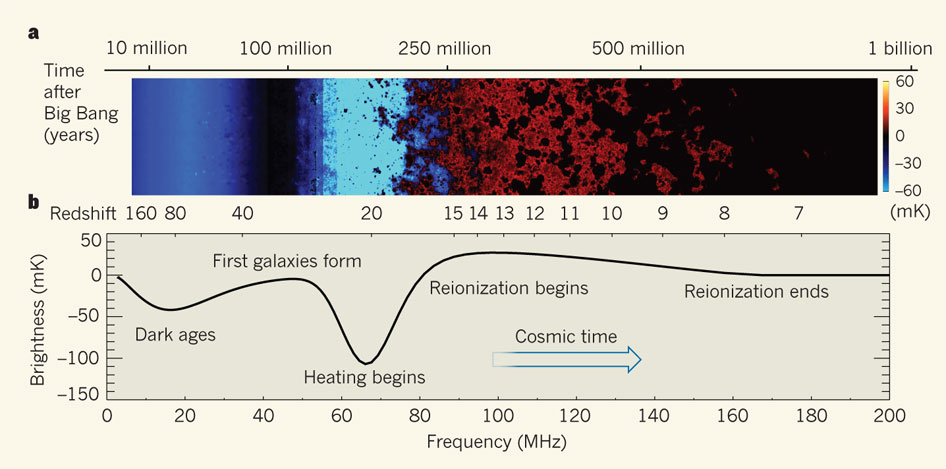
\includegraphics[width=0.95\linewidth]{Introduction/figures/pritchard_and_loeb_spectrum.jpg}
%\caption{Simulated \cm signal during the Dark Ages, Cosmic Dawn and Epoch of Reionization. (a) Spatial structure, and (b) average (global) spectrum. Image comes from Pritchard and Loeb \cite{pritchard_2010}. }
%\label{Fig:cm_hist}
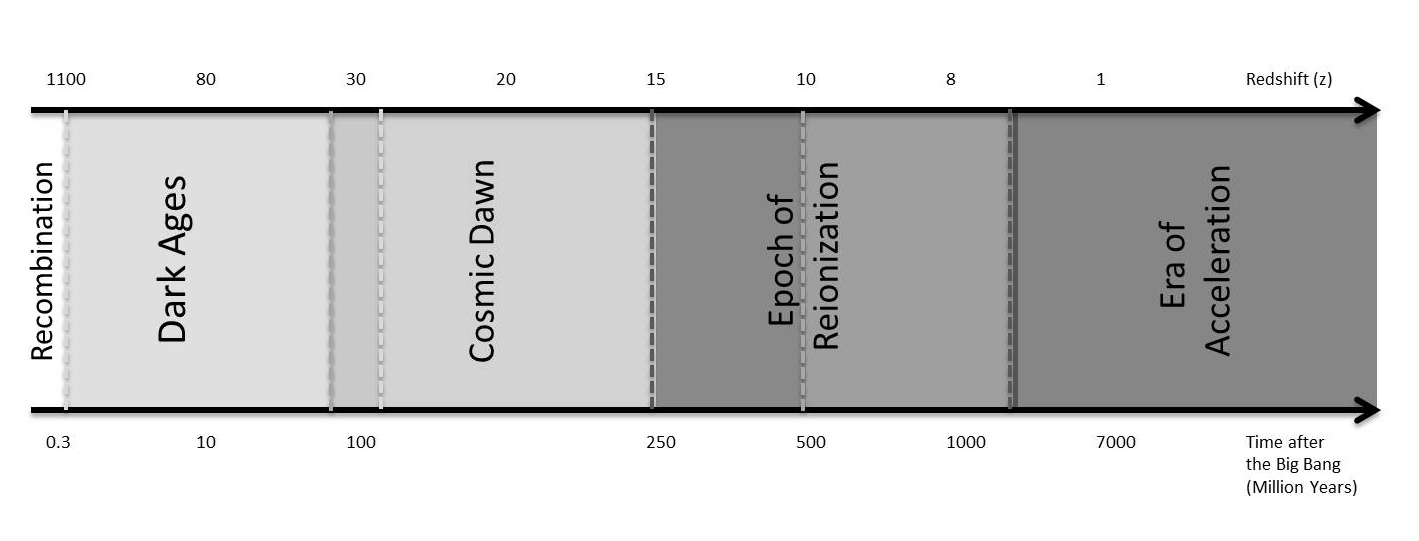
\includegraphics[width=0.95\linewidth]{Introduction/figures/timeline.jpg}
\caption{Timeline of cosmic history with redshift and approximate time since the Big Bang for the different cosmological eras. }
\label{Fig:hist}
\end{center}
\end{figure}

However, the recent development of \cm cosmology has provided a potential tool for measuring these eras of our history and filling in some of the blanks. There are a number of experiments which seek to utilize the \cm line to study the universe, as will be discussed in Section \ref{Sec:cm_expts}. These experiments focus on a number of cosmological eras, including the Dark Ages, Cosmic Dawn, and the Epoch of Reionization and Era of Acceleration that immediately follow them (see the timeline in Figure \ref{Fig:hist}). We will discuss the cosmological eras mentioned above in detail in Section \ref{Sec:IGMhist}.

In this thesis I focus on one particular experiment in \cm cosmology called SCI-HI, which observes the end of the Dark Ages and the Cosmic Dawn. In Chapter \ref{Ch:Intro} the science motivation for the experiment is outlined. A detailed description of the SCI-HI system is given in Chapter \ref{Ch:System}. Site selection for data collection with the SCI-HI system is discussed in Chapters \ref{Ch:RFI} and \ref{Ch:Iono}. Data analysis procedure and results from SCI-HI data collected in June 2013 are discussed in Chapter \ref{Ch:Data}. Plans for the future of SCI-HI are described in Chapter \ref{Ch:Conclude}. 

Working beyond the SCI-HI experiment, Appendix \ref{Ch:Planet} describes a strategy used to educate the public on \cm cosmology. This strategy is a planetarium show called $''$The Hydrogen Sky$''$. 



\section{Hydrogen \cm Science}

To set a background for \cm cosmology, we first need to understand the basic physics behind the signals that we are studying. There are four concepts that need to be outlined to facilitate this understanding. 

\begin{enumerate}

\item A review of the atomic states of Hydrogen and in particular the \cm hyperfine splitting of the ground state. 

\item An overview of spin temperature including a definition of the spin temperature of a cloud of neutral Hydrogen atoms and a discussion of how emission and absorption change the spin temperature. 

\item An overview of brightness temperature and how that temperature can change when it passes through a cloud of Hydrogen gas. 

\item A definition of the relationship between spin temperature, brightness temperature, and the opacity of a cloud of Hydrogen gas. 

\end{enumerate}

\begin{figure}[htb]
\begin{center}
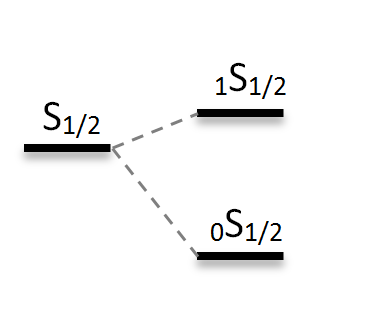
\includegraphics[width=0.6\linewidth]{Introduction/figures/1s_spin_states.png}
\caption{Simple atomic state diagram representing the hyperfine energy splitting of the Hydrogen ground state. }
\label{Fig:spin_states}
\end{center}
\end{figure}


\subsection{Hydrogen Atomic States}

The Hydrogen atom is the simplest atom, with only one proton and one electron. The proton and electron each have a spin $s_p,s_e = \pm \frac{1}{2}$. Interactions between the two spins lead to a splitting of the Hydrogen ground state into two energy levels. Using the Hamiltonian of a two spin system, we can calculate the eigenstates of the atom. These eigenstates can be written in terms of the spin state of the proton and electron ($| s_p, s_e \rangle$) as:

\begin{equation}
| 1 \rangle = | + \frac{1}{2}, + \frac{1}{2} \rangle 
\end{equation}
\begin{equation}
| 2 \rangle = | - \frac{1}{2} , - \frac{1}{2} \rangle 
\end{equation}
\begin{equation}
| 3 \rangle = \frac{1}{\sqrt{2}} (| + \frac{1}{2}, - \frac{1}{2} \rangle + |- \frac{1}{2}, + \frac{1}{2} \rangle) 
\end{equation}
\begin{equation}
| 4 \rangle = \frac{1}{\sqrt{2}} (| + \frac{1}{2}, - \frac{1}{2} \rangle - |- \frac{1}{2}, + \frac{1}{2} \rangle)
\end{equation}


States $| 1 \rangle$, $| 2 \rangle$, and $| 3 \rangle$ correspond to the higher energy eigenvalue, while state $| 4 \rangle$ corresponds to the lower energy eigenvalue. The energy difference between the two eigenstates is called $''$hyperfine splitting$''$, and has a value $E = h \nu_{10}$, where $\nu_{10}=1420.405 MHz$ and $\lambda_{10} = c /\nu_{10} = 21 \; cm$ \cite{townsend2000}. 

Figure \ref{Fig:spin_states} shows a graphical representation of the energy levels of these two spin states, where atomic quantum number notation is used to represent the states. In this notation the azimuthal angular momentum ($l$) is represented by the letter ($S$ means that $l=0$). The sub-script after the letter is the total angular momentum of the electron ($j=l+s$), where $s$ is the spin angular momentum of the electron. The sub-script before the letter is the total spin angular momentum ($F=0,1$) of the atom. 


\subsection{Spin Temperature (\ts)}

When working with a cloud of Hydrogen atoms rather than a single atom, we need to compare the number of atoms in each of the two hyperfine states. To do this, we define a spin temperature using Boltzmann's law for a cloud in thermodynamic equilibrium. Spin temperature (\ts) is defined using the ratio of the the two states $n_1/n_0$. The factor of 3 in Equation \ref{Eq:T_s} comes from the ratio of eigenstates for the different spin energy levels of the ground state of Hydrogen (3:1) \cite{field_1958}. 

\begin{equation}\label{Eq:T_s}
\frac{n_1}{n_0} \equiv 3 e^{- h \nu_{10} / kT_S} = 3 e^{-T_*/T_S}
\end{equation} 


\subsection{Emission and Absorption} \label{Sec:dT_S}

Change of the spin temperature occurs through emission and absorption of photons whose energy matches the transition energy between the two spin states. Transitions occur when the atom either spontaneously emits a photon or is induced to emit or absorb a photon due to external forces. These transitions can be described using a differential equation (Equation \ref{Eq:dn}) \cite{furlanetto_2006}, and each type of transition has a different rate coefficient $X^m_{ij}$. The rate coefficient notation here is: (a) the type of transition, m, (b) the initial state of the atom, i, and (c) the final state of the atom, j. 

\begin{equation} \label{Eq:dn}
\Big( \frac{d n_i}{dt} \Big)_m = X^m_{ij} n_i
\end{equation}

If the cloud is in equilibrium, the rates of change are equal, holding $n_{total} = n_0 + n_1$ constant. So $d n_0/dt = d n_1 /dt$, allowing us to calculate the spin temperature using Equation \ref{Eq:sn} \cite{field_1958}. 

\begin{equation} \label{Eq:sn}
n_0 \sum^m X^m_{01} = n_1 \sum^m X^m_{10}
\end{equation}

\subsubsection{Spontaneous Emission}

Spontaneous emission due to a transition between the spin states is caused by quantum interactions with the electromagnetic environment. Because the spin transition is a forbidden one, the lifetime of the higher energy (triplet) state is over 10 million years. The rate coefficient for sponaneous emission is the Einstein A coefficient ($X^A_{10} = A_{10}$), defined using Equation \ref{Eq:A_10}, where $\beta$ is the Bohr magneton \cite{field_1958}. 


\begin{equation} \label{Eq:A_10}
A_{10} = \frac{64 \pi^4 \beta^2}{3 h \lambda^3_{10}} = 2.85 x 10^{-15} sec^{-1}
\end{equation}


\subsubsection{Absorption and Stimulated Emission}

Since absorption and stimulated emission are transitions which depend on external triggers, they can occur at a higher rate than spontaneous emission. In the types of Hydrogen gas clouds that we are considering, there are three primary triggers: (a) \cm radiation, (b) baryon collisions, and (c) optical radiation \cite{field_1958}. 

\paragraph{\cm Radiation}

Incident radiation from an external source of \cm photons such as the Cosmic Microwave Background (CMB) will trigger absorption and stimulated emission. The rate coefficients of absorption and stimulated emission are set by the Einstein B coefficients ($X^R_{01} = B_{01} I_\nu$ and $X^R_{10} = B_{10} I_{\nu}$), where $I_{\nu}$ is the intensity of the external radiation. Since the CMB is a Blackbody, we know that $B_{10} I_{\nu} = A_{10} \lambda^2 I_{\nu}/ h \nu_{10}$. Also, the relative number of eigenstates for the two spin states means that $B_{01} = 3 B_{10}$ \cite{field_1958}. 


\paragraph{Baryon Collisions}

Collisions between the atoms and electrons in a Hydrogen gas cloud causes transitions described by coefficients $X^m_{01} = C_{01}$ and $X^m_{10} = C_{10}$. Because the system is in thermodynamic equilibrium, we can define a kinetic temperature (\tk) using the transition rate coefficients \cite{field_1958}. 

\begin{equation}
\frac{C_{01}}{C_{10}} \equiv 3 e^{-T_*/T_K}
\end{equation}

\paragraph{Optical Radiation}

Transitions to and from higher energy states  of the Hydrogen atom due to optical radiation will also cause transitions between spin states. This is known as the Wouthuysen-Field Mechanism \cite{wouthuysen_1952}\cite{field_1958} and will be discussed in greater detail in Section \ref{Sec:WFM}. For now, we'll just define an optical brightness temperature ($T_L$). This gives us Equation \ref{Eq:lcoef}, where the transition rate coefficients are $L_{01} = X^L_{01}$ and $L_{10} = X^L_{10}$ \cite{field_1958}. 

\begin{equation} \label{Eq:lcoef}
\frac{L_{01}}{L_{10}} = 3 e^{-T_*/T_L}
\end{equation}

\subsubsection{Spin Transition Rate Equation}

To calculate the spin temperature we combine the contributions from each of the sources of emission and absorption. Using the four sources described in the previous section, we get an expansion of Equation \ref{Eq:sn} for Hydrogen gas in equilibrium.

\begin{equation}\label{Eq:sns}
n_1(A_{10} + B_{10} I_\nu + C_{10} + L_{10}) = n_0 (B_{01} I_\nu + C_{01} + L_{01})
\end{equation}

By rearranging and using Equation \ref{Eq:T_s} to substitute for $n_1/n_0$, we get a direct relationship between the transition rates and the spin temperature. 

\begin{equation}
\frac{n_1}{n_0} = 3 e^{-T_*/T_S} = \frac{B_{01} I_\nu + C_{01}+ L_{01}}{A_{10}+ B_{10} I_\nu + C_{10} +L_{10}}
\end{equation}

Since $T_* = 68.1 mK$ and $T_S \gg T_*$, we can approximate the exponentials ($e^{-T_*/T} \simeq 1-T_*/T$) and rearrange to get Equation \ref{Eq:dT_s}. In this equation, the coupling coefficients are $x_K = T_* C_{10}/A_{10} T_K$ and $x_L = T_* L_{10} / A_{10} T_L$, and $T_R$ is the incident \cm radiation temperature \cite{field_1958}.

\begin{equation}\label{Eq:dT_s}
T_s \cong \frac{T_{R} + x_K T_{K} + x_{L} T_{L}}{1+x_K +x_{L}}
\end{equation}


\subsection{Brightness Temperature (\tb)}

The primary sources of incident radiation for Hydrogen gas clouds are Blackbody sources such as the CMB. These Blackbody sources have a spectral energy distribution ($B_\nu (T)$) defined by the Planck spectrum in Equation \ref{Eq:I_nu}. For long wavelengths, we use the Rayleigh-Jeans approximation ($B_{\nu} (T) \simeq (2 k \nu^2 / c^2) T$) to give us a brightness temperature ($T_b (\nu)$) \cite{carroll2007}. 

\begin{equation} \label{Eq:I_nu}
I_{\nu} (T) = B_{\nu}(T) = \frac{ 2 h \nu^3 / c^2}{e^{h \nu / k T}-1}
\end{equation}


\subsubsection{Change in Brightness Temperature}

Brightness temperature will change as the light travels through the universe. Such change can be caused by the expansion of the universe or by radiation sources and sinks such as gas clouds. Expansion of the universe simply causes the brightness temperature at each frequency to change at a rate proportional to the expansion rate ($a$). 

In comparison, radiation sources and sinks cause a frequency dependent shift in the brightness temperature. The rate of change of the brightness temperature is represented mathematically as a cloud opacity (\tu). Using opacity allows us to write the brightness temperature after passing through a radiation source using Equation \ref{Eq:T_bf}, where $T_{S}$ is the source temperature and $T_{R}$ is the original brightness temperature when it enters the source. As observers, what we actually care about and can measure is $\delta T_b (\nu) = (T_b (\nu))_{final} - T_R  (\nu)$. 

\begin{equation}\label{Eq:T_bf}
(T_b (\nu))_{final}= T_{S} (\nu) (1-e^{-\tau_\nu}) +T_{R} e^{-\tau_\nu}
\end{equation}



\subsection{Opacity ($\tau_\nu$)}

The change in brightness temperature caused by passing through a cloud of gas is determined by the cloud's opacity at a given frequency. Opacity (\tu) is defined as an integral along a line of sight through the cloud of the absorption rate of photons at the frequency $\nu$. The opacity for Hydrogen gas is defined for frequencies ($\nu \approx \nu_{10}$) using Equation \ref{Eq:tau}, where $\phi (\nu)$ is the line profile of the Hydrogen \cm spectral line at each position along the line of sight.

\begin{equation} \label{Eq:tau}
\tau_{\nu} = \frac{3 c^2 A_{10}}{8 \pi \nu^2 } (1-e^{-T_*/T_S}) \int ds \; \phi (\nu) n_0(s)
\end{equation}

 The line profile must have $\int \phi(\nu) d \nu = 1$ at each position. Meanwhile, $n_0 (s)$ is the number of Hydrogen atoms at each position that are in the spin 0 state \cite{furlanetto_2006}. In order to determine $n_0 (s)$ and $\phi (\nu)$ at each position, we need to know the details of the Hydrogen gas cloud. 



\section{The Intergalactic Medium (IGM)}\label{Sec:IGM}

The Intergalactic Medium (IGM) can be modelled as a Hydrogen gas cloud. Using the physics discussed in the previous section, we know that a cloud changes the brightness temperature of photons from the Cosmic Microwave Background (CMB) as they pass through the cloud. Therefore, the modified brightness temperature has a spectrum in frequency and space that depends on the history of the IGM. To make a prediction of this spectrum, we need a model of the history of the IGM during the time periods that we want to study. This model allows us to calculate the predicted \ts and \tu for the IGM. 


\subsection{IGM Fundamentals}

\subsubsection{Opacity ($\tau_\nu$)}

To calculate the opacity of the IGM, we need to use Equation \ref{Eq:tau} with the appropriate distribution of Hydrogen atoms in the lower spin state ($n_0$). The distribution, defined as $N_{HI} = 4 \int ds \; \phi(\nu) n_0(s)$, is the column density of Hydrogen gas. The factor of 4 in the column density comes from the total number of eigenstates in the ground state of Hydrogen. The column density can also be written as the fraction of Hydrogen that is neutral ($x_{HI}$) times the number of Hydrogen atoms along the line of sight ($n_H (z)$) times the line of sight ($s$).

With all of these factors, we can re-write the opacity as shown in Equation \ref{Eq:tau_approx}, where $(1+\delta)$ is the matter density at a given position relative to the average matter density. In addition, $dv_{\parallel}/dr_{\parallel}$ is the gradient of proper velocity along the line of sight and $H(z)$ is the Hubble parameter \cite{furlanetto_2006}. 

\begin{equation} \label{Eq:tau_approx}
\tau_{\nu} \approx 0.0092 (1+\delta) (1+z)^{3/2} \frac{x_{HI}}{T_S} \Big[ \frac{H(z)/(1+z)}{dv_{\parallel}/dr_{\parallel}} \Big] Kelvin
\end{equation} 



\subsubsection{Brightness Temperature Change (\dtb)}

As long as the opacity is small ($\tau_\nu \ll 1$), we can approximate $e^{-\tau_\nu}$ as $(1-\tau_\nu)$. As will be discussed in Section \ref{Sec:IGMhist}, this low opacity condition is expected to hold true during the eras of interest. Low opacity is due to the fact that the spin temperature is increasing with time during those eras and $\tau_\nu$ is inversely proportional to the spin temperature (see Figures \ref{Fig:da_global} and \ref{Fig:cd_global}). Therefore, we can write the change in brightness temperature of CMB photons due to passing through the IGM using Equation \ref{Eq:dT_b}, where \tg is the CMB photon temperature, which also acts as the incident radiation temperature ($T_R$) in Equation \ref{Eq:dT_s} \cite{furlanetto_2006}. 

\begin{equation}\label{Eq:dT_b}
\delta T_b = \frac{T_S - T_\gamma}{1+z}(1-e^{-\tau_\nu}) \approx 9 (1+\delta) (1+z)^{1/2} \Big(1-\frac{T_\gamma}{T_S}\Big) x_{HI} \Big[ \frac{H(z)/(1+z)}{dv_{\parallel}/dr_{\parallel}} \Big] mK
\end{equation}



\begin{figure}[htb]
\begin{center}
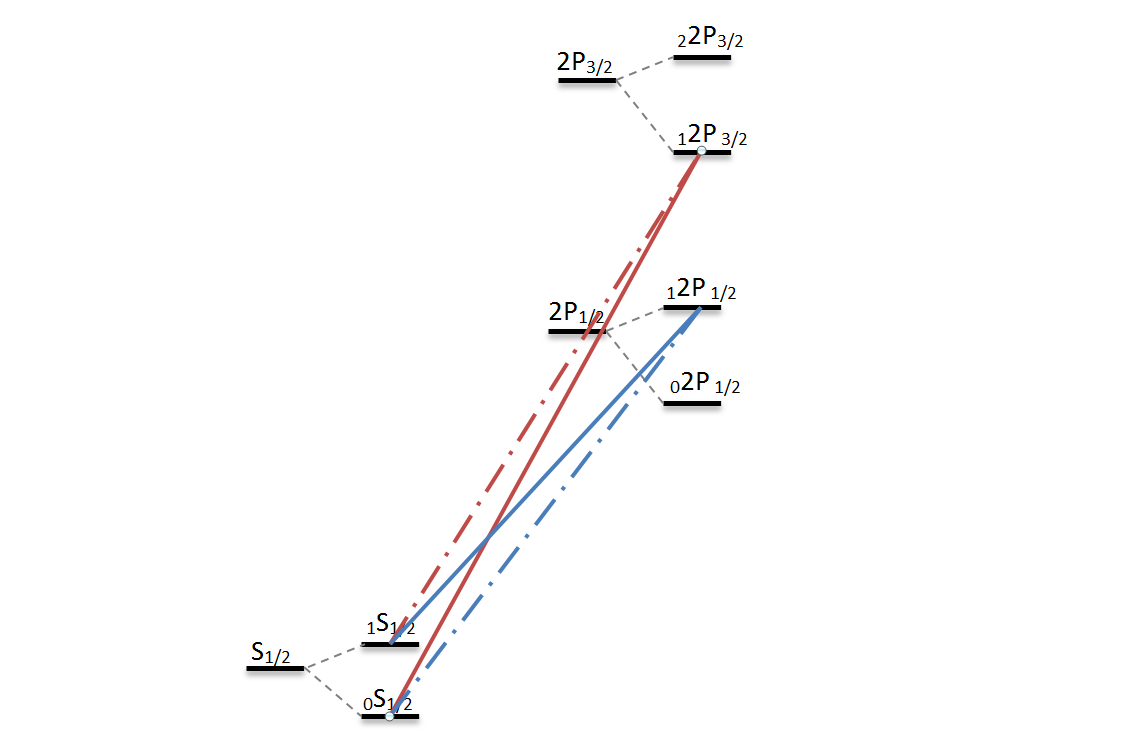
\includegraphics[width=0.95\linewidth]{Introduction/figures/wfm_states.png}
\caption{Simple atomic state diagram for the Wouthuysen-Field Mechanism. The pathway in blue corresponds to a $n_1 \rightarrow n_0$ transition while the pathway in red corresponds to a $n_0 \rightarrow n_1$ transition. Solid lines are the stimulated emission pathways, while the dashed lines are the absorption pathways.}
\label{Fig:wfm_states}
\end{center}
\end{figure}


\subsection{Wouthuysen-Field Mechanism}\label{Sec:WFM}

Given that the spin temperature of the IGM is a significant term in the brightness temperature equation, we need to understand how it can vary over time. As discussed in Section \ref{Sec:dT_S}, the spin temperature of Hydrogen in the IGM is coupled to three sources during its history. The first source is the CMB (\tg), which provides a source of external \cm radiation. The second source is the kinetic temperature of the gas (\tk), which characterizes the thermal motion of the atoms in the gas. The third and final source is external optical photons corresponding to transition energies between the ground and excited states of the Hydrogen atom. The most important transition for our purposes is the \lya transition. 

The mechanism for coupling between the Hydrogen spin temperature and \lya  photons is called the Wouthuysen-Field Mechanism \cite{wouthuysen_1952}\cite{field_1958}. To understand this mechanism, we must go back to the atomic states of the Hydrogen atom. Just as we've discussed for the \cm transition, external photons with an energy corresponding to the \lya  wavelength ($\lambda_{Ly-\alpha} = 121.6$ nm) can be absorbed by the atom. This induces a transition from the ground state of Hydrogen to its first excited state. The excited state is not stable, so the Hydrogen atom will eventually decay back to its ground state and emit a photon. However, conservation of angular momentum limits these stimulated emission transitions. 

Figure \ref{Fig:wfm_states} shows the possible transition chains for the \lya absorption and stimulated emission process. One transition chain occurs when the original $S_{1/2}$ state is the $F=0$ state, and can be written as $_0S_{1/2}$ $\rightarrow$ $_1P_{1/2}$ $\rightarrow$ $_1S_{1/2}$. The other transition chain occurs when the original $S_{1/2}$ state is the $F=1$ state, and can be written as $_1S_{1/2}$ $\rightarrow$ $_1P_{3/2}$ $\rightarrow$ $_0S_{1/2}$. 

So the absorption and stimulated emission of \lya photons redistributes the the neutral Hydrogen atoms in the ground state such that $n_{tot} = n_0 + n_1$ is unchanged but the spin temperature increases or decreases. The exact magnitude of the change in spin temperature will depend on the distribution of photons with wavelengths around the \lya wavelength. This is because the input photon frequency for $n_0 \rightarrow n_1$ is not identical to the input photon frequency for $n_1 \rightarrow n_0$ due to hyperfine splitting. 

Determining the rate of redistribution by the Wouthuysen-Field Mechanism requires the spectral distribution of \lya photons in the IGM and the \lya coupling coefficient. The spectral distribution of \lya photons is set by collisions within the IGM, and approximates a Blackbody curve with temperature $T_{Ly-\alpha} = T_K$. Meanwhile, the \lya  coupling term ($x_L = x_{\alpha}$) is proportional to the intensity of \lya  photons produced by external sources of light. The exact \lya  coupling coefficient is related to the rate of scattering of \lya  photons by Equation \ref{Eq:xa}, where $P_{\alpha}$ is the scattering rate \cite{furlanetto_2006}. 

\begin{equation}\label{Eq:xa}
x_{\alpha} = \frac{4 P_{\alpha} T_*}{27 A_{10} T_{\gamma}}
\end{equation}

Calculation of the scattering rate requires knowledge of the absorption cross section of photons ($\sigma_{\nu}$). It also requires knowledge of the intensity of incident radiation from external optical radiation sources ($J_{\nu}$). This is shown in Equation \ref{Eq:pa} \cite{furlanetto_2006}. Optical radiation sources present during different cosmological eras will be discussed in Section \ref{Sec:IGMhist}. 

\begin{equation}\label{Eq:pa}
P_{\alpha} = 4 \pi \int d\nu J_{\nu}(\nu) \sigma_{\nu}(\nu)
\end{equation}


\subsection{History of the IGM} \label{Sec:IGMhist}

\subsubsection{Initial Conditions}

In the early universe before galaxies came into existence, the entire universe was filled with a medium that was the progenitor of the IGM. From measurements of the Cosmic Microwave Background, we know that at $z \sim 1100$ the IGM was a nearly homogeneous gas of protons, free electrons, and atoms; most of which were neutral Hydrogen (HI) atoms. Within the gas were small inhomogeneities in the matter density that would eventually grow into galaxies, but the average gas density was high enough that collisions between baryons were common throughout the medium \cite{furlanetto_2006}. 

\begin{figure}[htb]
\begin{center}
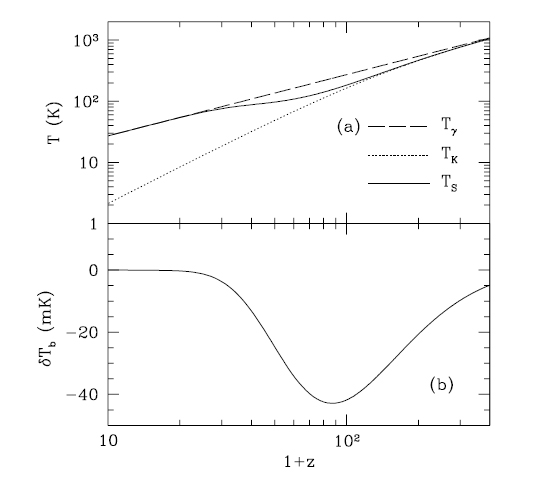
\includegraphics[width=0.95\linewidth]{Introduction/figures/dark_ages_global_spectrum.jpg}
\caption{(a) Plot of $T_S$, $T_\gamma$, and $T_K$ during the dark ages calculated from initial conditions given by the CMB and (b) $\delta T_b$ during the same period with only collisional coupling present. Plots come from Furlanetto et. al. \cite{furlanetto_2006}}
\label{Fig:da_global}
\end{center}
\end{figure}

\subsubsection{Dark Ages}

During the Dark Ages, adiabatic gas cooling and collisional coupling created structure in the spin temperature relative to the CMB temperature. Right after recombination ($z \sim 1100$), the IGM was dense enough for Compton scattering between CMB photons and free electrons in the IGM to set \tk$=$\tg$=$\ts. But as the universe expanded, the gas adiabatically cooled faster than the CMB. This led to thermal decoupling, so \tk decreased below \tg. 

When this thermal decoupling occurred, collisions between baryons in the IGM were still frequent enough to keep $x_K$ large. Therefore, the spin temperature began to drop below the CMB temperature. However, $x_K$ coupling gradually decreased as the rate of collisions between baryons decreased. Eventually, the spin temperature became exclusively coupled to the CMB temperature. 

The process of cooling and collisional decoupling created a dip in \ts, which most models predict should be centered around $z \sim 80 $ \cite{furlanetto_2006}. Figure \ref{Fig:da_global} shows one model prediction for the relevant temperatures including \tg, \tk, \ts and \dtb before star formation. 

\begin{figure}[htb]
\begin{center}
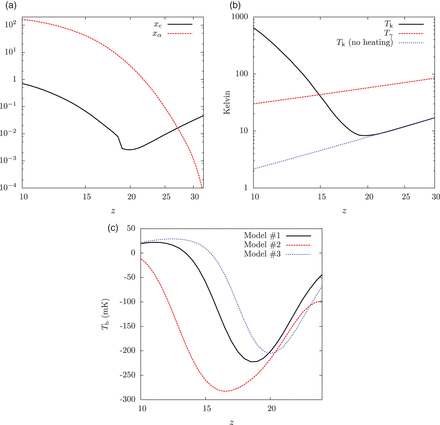
\includegraphics[width=0.95\linewidth]{Introduction/figures/ts_evolution.png}
\caption{Plots of (a) $x_K$ and $x_{\alpha}$, (b) $T_\gamma$ and $T_K$ with and without X-ray heating, and (c) $\delta T_b$ during the Cosmic Dawn for different models of star formation from Natarajan et. al. \cite{natarajan_2014}}
\label{Fig:cd_global}
\end{center}
\end{figure}

\subsubsection{Cosmic Dawn}

The beginning of the $''$Cosmic Dawn$''$ is defined as the time when the first stars in the universe began to form. During the Dark Ages, hierarchical structure formation led to more and more massive dark matter minihaloes. The first (PopIII.1) stars are believed to have formed in dark matter minihaloes with mass $\sim 10^6 - 10^8 M_{\odot}$, which $\Lambda$CDM simulations predict occurred around redshifts of $z \approx 20-30$ \cite{bromm_2013}. PopIII.1 stars had three major impacts on the IGM: (a) stars produced UV photons which ionized Hydrogen in the IGM, (b) UV photons also increased Wouthuysen-Field coupling and collisional coupling to the spin temperature (c) some of the first stars were X-ray sources, which heated the IGM and increased its kinetic temperature.

%\textcolor{red}{Add figure of HII bubbles from aravind's review paper's reference.}

Ionization by UV photons created bubbles of ionized Hydrogen (HII) around the stars. These bubbles gradually expanded and merged until the IGM was fully ionized. This process of ionization leads to the Epoch of Reionization, which will be discussed in the next section.

Meanwhile, UV photons included \lya  photons, which caused increasing coupling between \ts and \tk due to the Wouthuysen-Field Mechanism. The total amount of coupling from the first stars ($x_\alpha$), shown in Equations \ref{Eq:xa} and \ref{Eq:pa}, is related to the \lya  photon intensity $J_\alpha$. This photon intensity comes from the emissivity of \lya photons by the stars. Additional photon intensity comes from the emissivity of photons in other Lyman transitions which cascade down to affect the \lya  transition rate. Emissivity is heavily dependent on the rate of first star formation and the initial mass function (IMF) of PopIII.1 stars. Some models suggest that PopIII.1 stars may have a heavier IMF than is observed in the modern universe. If this is true, PopIII.1 stars would have produced more \lya  photons per star, changing the evolution of $x_\alpha$ \cite{natarajan_2014}. 

During this era of first star formation, X-ray photons were produced by two types of sources among the first PopIII.1 stars. One source of X-ray photons was electrons accelerated by supernovae to relativistic speeds. When these electrons undergo inverse Compton scattering, X-ray photons are produced. The other source of X-ray photons was high-mass X-ray binary stars, which occur when massive stars on the main sequence lose material through accretion onto a compact neighbor such as a neutron star, black hole or white dwarf star. These high energy photons heated the IGM through a combination of photoionization of Hydrogen or Helium atoms and collisions with IGM components. In most models of cosmic history, X-ray sources appear later than the first PopIII.1 stars \cite{furlanetto_2006}. 

Depending on the time delay between the appearance of the first PopIII.1 stars and the first X-ray sources, as well as the relative rates of X-ray heating and \lya coupling, the predicted variance of the average spin temperature over time is modified. The spin temperature is predicted to dip during the period where $x_K>0$ and \tk is less than \tg. However, by varying the model of first star formation that sets these two rates for PopIII.1 stars, the exact shape of the dip in the spin temperature will be modified. 

Most models predict a dip centered around $z\sim20$, with a width of $0 \leq z \leq 10$ and a depth of $0\leq \Delta T \leq 300 mK$. Figure \ref{Fig:cd_global} shows a few models of global \dtb$\;$ during the Cosmic Dawn, as well as some of the parameters that feed into the brightness temperature variance. These models were run by Aravind Natarajan using SIMFAST code \cite{simfast}\cite{21cmfast}\cite{natarajan_2014}.  

\begin{figure}[htb]
\begin{center}
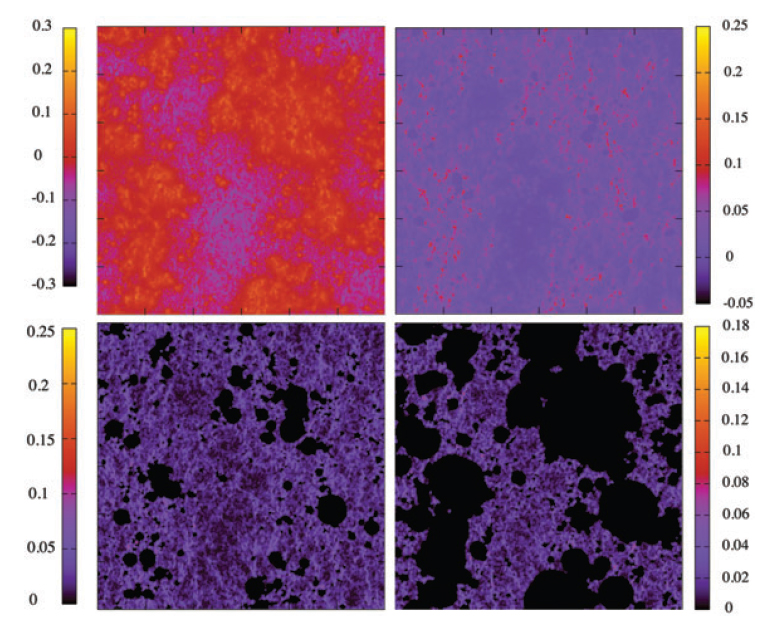
\includegraphics[width=0.95\linewidth]{Introduction/figures/reionization.jpg}
\caption{Snapshots at $z=$14,12,10,8 (from top left to bottom right) from a simulation run using SIMFAST from Natarajan et. al. \cite{natarajan_2014}. The simulation shows the expected \dtb signal in units of Kelvin during the Epoch of Reionization. }
\label{Fig:eor}
\end{center}
\end{figure}

\subsubsection{Epoch of Reionization (EoR)}

As the kinetic temperature of the IGM continued to rise, it reached the threshold where Equation \ref{Eq:dT_b} breaks down because the kinetic and spin temperatures of the IGM are large enough that the approximation used for \tu $\;$ is no longer applicable. At this point \dtb$\;$ reaches a maximum because of saturation of the signal. 

Propogation of X-ray and UV photons through the IGM also began to ionize the Hydrogen atoms, starting in regions near the galaxies and spreading gradually throughout the IGM (see Figure \ref{Fig:eor}). This period of time is also known as the Epoch of Reionization (EoR) because the IGM is resuming the ionized state that it had in the early universe. Since the brightness temperature of the \cm signal is also proportional to the amount of neutral Hydrogen ($x_{HI}$) present in the IGM, as shown in Equation \ref{Eq:dT_b}, the ionization process caused a gradual decrease in the average \cm signal. 

However, the gradual nature of the ionization means that there are interesting structures in the spatial distribution of the \cm signal during the EoR. The exact spatial distribution over time provides insight into the distribution of the PopIII.1 stars, since larger stars produce more ionizing photons compared to the number of \lya  photons \cite{furlanetto_2006}. 

\subsubsection{Era of Acceleration}

In the post-reionization universe, neutral Hydrogen gas in the IGM is limited to the regions around galaxies with a large column density. The minimum column density ($N_{HI}>10^{21} cm^{-2}$) is set by the minimum density required to self-shield the gas from ionizing UV photons. This gas can still be mapped using the \cm signal, but the magnitude of the signal is much smaller than in previous eras. 

In this regime, mapping of the spectral structure can be done through intensity mapping. Intensity mapping is a process by which the signal from neutral Hydrogen can be measured in aggregate around many galaxies. This is done with data that is collected in large voxels. Each voxel contains many galaxies and the \cm signal that is measured is the sum of the \cm signal from all the galaxies in that voxel \cite{masui_2012}. This period of cosmic history is called the Era of Acceleration, because it was during this time ($z \sim 1$) that the expansion of the universe began to accelerate. 

\section{Measuring the \cm Signal}

After passing through the IGM at a given time, the \cm photons travel toward the Earth. As they travel, the photons' frequencies are redshifted ($\nu_{meas} = \nu_{10}/(1+z)$) from their original frequencies. This shift allows us to measure a spectrum $\delta T_b (\nu)$, where $\nu$ is the frequency at which the signal is measured, corresponding to the redshift where the signal was produced. 

Measurements of the \cm spectrum are classified in two types. The first type are measurements of the sky-averaged spectrum (\avgdtb). The second type are measurements of the spatial fluctuations in the \cm spectrum ($\delta_{T_b} (\theta, \phi, \nu) =  \delta T_b (\theta, \phi, \nu)/ T_b (\nu)$) using the power spectrum of the fluctuations ($ \tilde{\delta}_{T_b} ( \vec{k} )$) \cite{natarajan_2014}. This thesis focuses on a measurement of the first type, a sky-averaged spectrum. 

\begin{figure}[htb]
\begin{center}
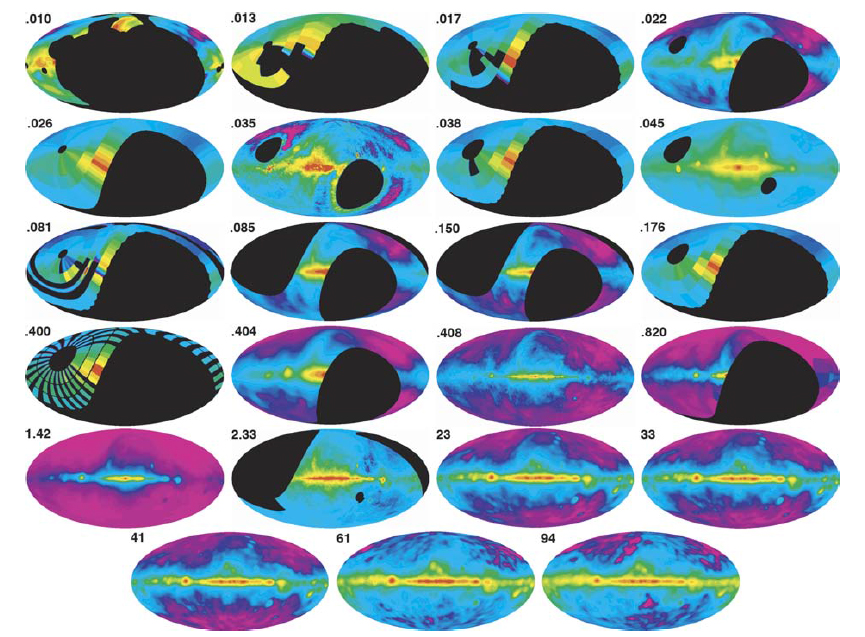
\includegraphics[width=0.95\linewidth]{Introduction/figures/GSM_maps.jpg}
\caption{Plots of radio sky measurements used to construct the Global Sky Model \cite{GSM_model} of radio foregrounds. The number in the upper left corner of each plot is the frequency (in $GHz$) at which the map data was collected, while the color scale is the log of the sky temperature in Kelvin.}
\label{Fig:GSM_maps}
\end{center}
\end{figure}


\subsection{Non-Cosmological Foregrounds} \label{Sec:gsm_fore}

One of the greatest challenges of making any \cm measurements is the presence of foreground sources in the sky. Foreground sources are astrophysical objects which emit in the low frequency radio band ($\nu \leq \nu_{10}$), interference from Earth's ionosphere, and radio frequency interference (RFI) from man-made sources. I will discuss RFI in Chapter \ref{Ch:RFI} and ionospheric impacts in Chapter \ref{Ch:Iono}, so in this section I will focus on astrophysical foregrounds. 

For $\nu \leq \nu_{10}$ the dominant astrophysical foreground is synchrotron radiation from the Milky Way Galaxy. This radiation comes from free electrons in the Milky Way Galaxy and has a strongly downward sloping spectrum near the Galactic Poles \cite{furlanetto_2006}. 

\begin{equation}\label{Eq:T_sky_approx}
T_{sky} \approx 180 \Big( \frac{\nu}{180 MHz} \Big)^{-2.6} K
\end{equation}

Maps of astrophysical foregrounds have been made at a number of frequencies, including the $''$Haslam$''$ map at $408 MHz$ and the WMAP maps (after removal of the CMB signal) at 23,33,41,61 and $94 GHz$. These maps are shown in Figure \ref{Fig:GSM_maps}. A model of the foregrounds from $10 MHz-100 GHz$ was constructed using the maps, as outlined in de Oliveira-Costa et al \cite{GSM_model}. This sky model is commonly used for foreground assessment and even calibration by \cm experiments. Section \ref{Sec:model} details how the GSM model is used in the SCI-HI project.


\subsection{Average (Global) Frequency Spectrum (\avgdtb)} \label{Sec:avgdtb}

To make a measurement of \avgdtb, experiments measure the total sky brightness temperature spectrum ($T_{Sky}$) over a wide range of frequencies. The combination of signals collected by an antenna is given in Equation \ref{Eq:T_ant_sky}, where $T_{fg}$ is the astrophysical foreground signal, $T_{RFI}$ is the man-made signal, $T_{sys}$ is the system temperature, and \tb is the brightness temperature from the CMB. 

\begin{equation} \label{Eq:T_ant_sky}
T_{Ant} = T_{fg} + T_b +T_{sys}+T_{RFI} = T_{Sky} + T_{sys}
\end{equation}

The system temperature ($T_{sys}$) will be a combination of thermal noise and instrument noise. Thermal noise is set by the radiometer equation ($T_{thermal} = T_{ant}/\sqrt{BW \tau}$), where $BW$ is the system bandwidth and $\tau$ is the integration time \cite{carroll2007}. Instrument noise comes from the electronics in the system (such as the amplifiers). 

Extracting the \cm brightness temperature spectrum requires removing all of the other terms in the data. Different strategies have been proposed for removing these signals, but all of them rely on the fact that the other signals have a different type of spectral structure than the \cm signal. I will discuss one such strategy for foreground removal with the SCI-HI experiment in Section \ref{Sec:fore}. 


\subsection{Fluctuation Power Spectrum ($ \tilde{ \delta}_{T_b}  ( \vec{k} )$)}

Like \avgdtb$\;$ experiments, power spectrum measurements are also dominated by foregrounds. Unlike \avgdtb$\;$ experiments, these foregrounds are primarily specific galactic and extragalactic point sources. These sources have a brightness temperature spectrum that can be fitted with a power law; although each point source has a different power law coefficient. 

There are a number of different specific foreground removal strategies that have been developed, including principal component analysis \cite{masui_2012}\cite{switzer_2013}. All of these strategies rely on the removal of the dominant foregrounds through their smooth spectra. The \cm signal is left behind when the foregrounds are removed because it will have complex structure in frequency. This is because each frequency corresponds to the signal from a different set of galaxies in the intensity map. 



\section{Hydrogen \cm Cosmology Experiments} \label{Sec:cm_expts}

There are a number of experiments whose goal is measurement of the \cm global signal or power spectrum. Some of these experiments are currently gathering data, while others are still under development. Preliminary constraints on \cm signals have been placed for several cosmological eras using current experiments. Future measurements should continue to tighten constraints on the \cm global signal and \cm power spectrum during the Dark Ages, Cosmic Dawn, Epoch of Reionization and Era of Acceleration. 


\subsection{Global (All-Sky Average) Experiments}

Experiments that are trying to measure \avgdtb$\;$ focus on redshifts where \avgdtb is large and/or has a large first derivative. This is predicted to occur during the Dark Ages, Cosmic Dawn, and the Epoch of Reionization. EDGES \cite{bowman_2008} is a single antenna experiment focused on frequencies from $100-200 MHz$. It has placed limits on the duration of reionization by setting a minimum width for the \cm global signal emission bump during the Epoch of Reionization (EoR). Similar experiments, such as BIGHORNS\cite{bighorns}\cite{sokolowski_2015}, are also under development and are targeting the EoR spectrum.  

Meanwhile, LEDA \cite{leda}\cite{bernardi_2014} and DARE \cite{burns_2011} are currently under development, and are targeting the Dark Ages and Cosmic Dawn. LEDA is designed to operate on the ground using a combination of an interferometer and a single antenna, while DARE intends to launch a satellite in orbit around the moon with a single antenna. 

Both of these experiments have large budgets of over 1 million dollars and require significant resources and technology development. In contrast, the EDGES experiment is on a much smaller scale and can be deployed in the field with minimal infrastructure.

\subsubsection{SCI-HI Experiment}

We were inspired by the EDGES experiment to develop a similar system that focuses on a different part of the \cm spectrum ($40 \leq \nu \leq 130 MHz$), going after the Cosmic Dawn signal. This experiment is the SCI-HI experiment, and is the main focus of the rest of this thesis. 


\subsection{Mapping Experiments}

Experiments which seek to measure the \cm power spectrum are typically many-element interferometers, each experiment with its own antenna design and configuration. Early projects, including the GMRT-EoR \cite{paciga_2013} project, made use of existing telescopes to make measurements. Meanwhile, a number of projects were designed and constructed such as the Precision Array for Probing the Epoch of Reionization (PAPER) \cite{pober_2013}\cite{jacobs_2014}, the Murchison Widefield Array (MWA) \cite{bernardi_2013}\cite{tingay_2012}, and the Low Frequency Array for Radio Astronomy (LOFAR) \cite{jelic_2014}\cite{lofar}. These projects have put first constraints on the power spectrum during the EoR. Future projects targeting the EoR signal include the Hydrogen Epoch of Reionization (HERA) \cite{hera}\cite{bernardi_2014} array and the Square Kilometer Array (SKA) \cite{ska}.

Beyond the EoR projects, there are a number of power spectrum projects focusing on lower redshifts during the Era of Acceleration. The \cm signal targeted by these projects is much smaller than the EoR signal, but the foregrounds at these frequencies are also much smaller. First constraints on the power spectrum at ($z \sim 0.8$) were placed by the GBT-IM project \cite{masui_2012}\cite{switzer_2013}, which used the Robert C. Byrd Green Bank Telescope to make a map of a few degree patch of sky and construct a power spectrum from that map. 

As with the EoR experiments, full sky mapping at later times also requires a dedicated instrument. One such instrument is the Canadian Hydrogen Intensity Mapping Experiment (CHIME) \cite{shaw_2014}\cite{chime}, currently under development. CHIME uses a unique cylindrical interferometer design to map the sky. Several other experiments are in earlier stages of planning and development, including the TIANLAI project in China and the HIRAX project in South Africa. Appendix \ref{Ch:Planet} includes some discussion of the Green Bank Telescope and CHIME, and how they were used in an outreach project educating the public on \cm cosmology. 

